\edef\mychapter{Inequalities}
\edef\mychapterdate{July 7, 2024}

\chapter{\mychapter}

\section{Basic Inequalities}
\subsection{Increasing or Decreasing}
In this section, we will introduce the notion of an increasing or decreasing function. Generally, this concept is pretty easy to visualize on a plot, for example, in figure \eqref{fig:inc}, we can observe an increasing function.
\begin{figure}[h]
\centering
	\begin{tikzpicture}
		\begin{axis}
			\addplot[blue, thick,domain=-1:1]{x^3};
		\end{axis}
	\end{tikzpicture}
	\caption{Plot of $x^3$.}
	\label{fig:inc}
\end{figure}
Then in figure \eqref{fig:dec}, we can observe $-x^3$ is an example of a decreasing function.
\begin{figure}[h]
\centering
	\begin{tikzpicture}
		\begin{axis}
			\addplot[blue, thick,domain=-1:1, samples=100]{-x^3};
		\end{axis}
	\end{tikzpicture}
	\caption{Plot of $-\ln(x)$.}
	\label{fig:dec}
\end{figure}
However, these declarations are only applied to a specific subset of all possible functions.
\begin{figure}[h]
\centering
	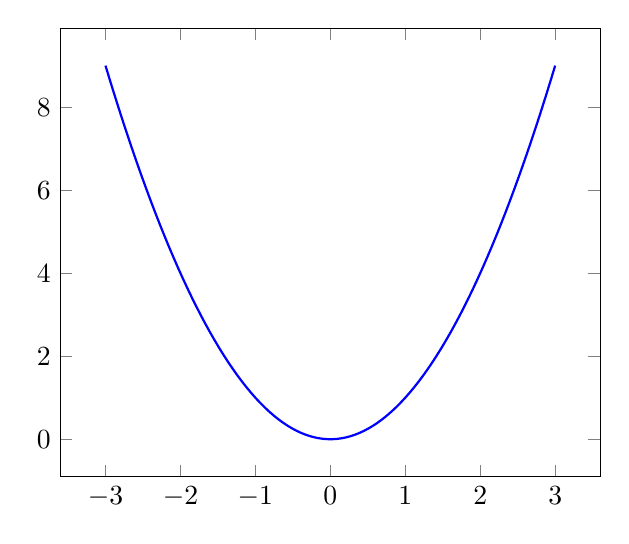
\begin{tikzpicture}
		\begin{axis}
			\addplot[blue, thick,domain=-3:3, samples=100]{x^2};
		\end{axis}
	\end{tikzpicture}
	\caption{Plot of $x^2$.}
	\label{fig:neith}
\end{figure}
In figure \eqref{fig:neith}, we can observe a function that is neither increasing nor decreasing. But it is here that we note that whether a function is increasing or decreasing also heavily depends on what domain we define the function on. Had we restricted the domain to $x\ge0$ in figure \eqref{fig:neith}, we would get an increasing function.

Now, with this basic intuition, let's define these ideas more rigorously with mathematics.

\begin{define}
Let $f:\real\to\real$\footnotemark be an increasing function. Then $a<b$ implies $f(a)\le f(b)$.
\label{def:inc}
\end{define}
\footnotetext{Technically, this is defined for any ordered set with a notion of "bigness", but for this introductory course, we will restrict ourselves just to $\real$, or subsets of $\real$.}
\begin{define}
Let $f:\real\to\real$ be a decreasing function. Then $a<b$ implies $f(a)\ge f(b)$.
\end{define}

Now, had we exchanged the non-strict inequalities for strict inequality, so $a<b$ implies $f(a)<f(b)$ and $f(a)>f(b)$, we would get the definition for a \textbf{strictly increasing} and \textbf{strictly decreasing} function, respectively.
Now it must be mentioned that with the mathematical machinery that we have, proving a real function is decreasing or increasing can be difficult in general.
We will start to develop ways to determine this in a later lecture.

\subsection{Solving Basic Inequalities}
\begin{ex}
	In this example, let's solve the inequality
	$$12 > 7-2y$$
	This might seem very obvious to many of you, but in this example, I will attempt to demonstrate a slightly different way of thinking about this.
	Define a function $f:\real\to\real$ such that $f(x)=x-7$.
	By plotting the function on an axis, $f$ is clearly increasing.
	Therefore,
	$$12 > 7-2y$$
	implies
	\begin{align*}
		f(12)  &> f(7-2y) \\
		(12)-7 &> (7-2y)-7 \\
		-7     &> -2y
	\end{align*}

	Then define a different function $g:\real\to\real$ such that $g(x)=-\frac{1}{2}x$.
	Since this is a decreasing function,
	$$-7>-2y$$
	implies
	\begin{align*}
		g(-7) 				&< g(-2y) \\
		-\frac{1}{2}(-7) 	&< -\frac{1}{2}(-2y) \\
		\frac{7}{2}			&< y
	\end{align*}
	hence we conclude every $y$ such that
	$$y\in\paren{-\infty,\frac{7}{2}}$$
	satisfies our inequality since the steps we took to arrive at this result are completely reversible.
	\label{ex:basicineq}
\end{ex}

\begin{ex}
	Let's solve the inequality
	$$x^2+3x\le-2.$$
	By the same technique as shown in example \eqref{ex:basicineq}, we show
	$$x^2+3x+2\le0.$$

	\begin{figure*}
		\centering
		\resizebox{0.6\textwidth}{!}{\includegraphics{chapters/assets/ineq/quadplots.png}}
		\caption{}
		\label{fig:quad}
	\end{figure*}
	Looking at the inequality, we see what values of $x^2+3x+2$ sit on or above the $x$-axis (since our inequality is not strict) when plotted.
	In general, when we plot a quadratic as in figure \eqref{fig:quad}, we know there are a few options:
	\begin{enumerate}
		\item There are no solutions.
		\item There is one solution.
		\item There is a connected interval of solutions between the two zeros.
		\item There is a disjoint interval of solutions around the two zeros.
		\item Every real number satisfies the inequality.
	\end{enumerate}
	We can summarize these observations with the following:
	If the quadratic \textit{exactly} has two roots, then the inequality will be satisfied with a disjoint or connected interval in $\real$;
	if the quadratic has no roots (in $\real$), either the inequality has no solutions are every $x\in\real$ will satisfy;
	if the quadratic has one root, either the inequality will have one solution or every $x\in\real$ will satisfy.

	Let's see which scenario we have here.
	Finding the roots of this quadratic proceeds as follows:
	\begin{align*}
		x^2+3x+2	&=0
		(x+2)(x+1)	&=0
	\end{align*}
	hence
	$$x=\{-2,-1\}.$$
	Therefore, our desired solution set is either a connected or disjoint interval in $\real$.
	To figure out which one it is, we just need to test a point.
The easiest to test in this case is 0, but any point that isn't a root will suffice\footnote{A root will trivially satisfy or not satisfy depending on the choice of inequality sign}.
Substituting 0 gives
	$$(0)^2+3(0)+2=2\not\le 0$$
	Since $0$ lies around the two roots, we arrive at
	$$x\in[-2,-1].$$
\end{ex}

\subsection{Absolute Values}
To facilitate our formal discussion of absolute values, let's give a rigorous definition.
\begin{define}
	For any $x\in \real$, let $|x|:=\max\{x, -x\}$
\end{define}

\begin{prop}
	Suppose $c, x \in \real$, then
	\begin{enumerate}
		\item $c < |x|$ if and only if $c<x$ or $c<-x$,
		\item $|x|<c$ if and only if $-c < x < c$.
	\end{enumerate}
\end{prop}
\begin{proof}
	Let's prove statement (1).
	Suppose $c< |x|=\max\{x, -x\}$, thus either
	$$c < x \jor c < -x.$$
	If $c < x$, then $c< x \le \max\{x, -x\}=: |x|$.
	Similarly, if $c < -x$.

	For statement (2), if $|x| :=\max\{x, -x\} < c$.
	Since
	$$x \le \max\{x, -x\} \jand x \le \max\{x, -x\},$$
	we have $x < c$ and $-x < c$, thus implying $-c < x < c$.
	Conversely, if $-c<x<c$, then $-x < c$ and $x < c$, thus $\max\{x, -x\} < c$.
\end{proof}

The proposition is true if we replace every strict inequality with a non-strict inequality, which follows similarly.

\begin{theorem}[Triangle Inequality]
	Suppose $x,y\in\real$, then
	$$|x|+|y|\ge |x+y|$$
	\label{thm:triangle}
\end{theorem}
\begin{proof}
	By the definition of the absolute value, observe
	$$-|x|\le x \le |x|$$
	$$-|y|\le y \le |y|$$
	Adding the two inequalities gives
	$$-(|x|+|y|)\le x+y \le |x|+|y|$$
	which implies
	$$|x+y|\le ||x|+|y||.$$
	Since $|x|+|y|\ge 0$,
	$$|x+y|\le |x|+|y|.$$
\end{proof}

\begin{cor}
	Suppose $x,y\in\real$, then
	$$||x|-|y||\le |x-y|$$
	\label{cor:invtri}
\end{cor}
\begin{proof}
	For this one, we are going to define the variable $a=x-y$.
	By theorem \eqref{thm:triangle},
	$$|a|+|y|\ge|a+y|=|x|.$$
	Therefore,
	$$|x-y|\ge |x|-|y|.$$
	Then letting $b=y-x$, by theorem \eqref{thm:triangle},
	$$|x|+|b|\ge|x+b|=|y|$$
	implying
	\begin{align*}
		|y-x|	&\ge|y|-|x|
		|x-y|	&\ge-(|x|-|y|)
		-|x-y|	&\le |x|-|y|.
	\end{align*}
	Therefore,
	$$-|x-y|\le |x|-|y|\le |x-y|$$
	implying
	$$|x-y|\ge ||x|-|y||.$$
\end{proof}

\section{Bounds}
\subsection{Bounded Functions}
\begin{define}
Let $f:\real\to\real$ be bounded above. Then there exists $M\in\real$ such that
for any $x\in\real$, $M\ge f(x)$.
\end{define}
\begin{define}
	Let $f:\real\to\real$ be bounded below. Then there exists $M\in\real$ such that for any $x\in\real$, $M\le f(x)$.
\end{define}
\begin{define}
	Let $f:\real\to\real$ be bounded. Then there exists $M>0$ such that for any $x\in\real$, $M\ge |f(x)|$, or equivalently, $f$ has an upper and lower bound.
\end{define}
Now, to present these concepts more visually, we examine the function $f(x)=\frac{\sin(x)}{x}$.
In figure \eqref{fig:upper}, we can see I've bound the function by $y=1.2,1.5,1.8$.
\begin{figure*}[h]
	\centering
	\resizebox{0.6\textwidth}{!}{\includegraphics{chapters/assets/ineq/upperbound.png}}
	\caption{}
	\label{fig:upper}
\end{figure*}
Now, since the definition of a bounded function only requires a bound to exist, we could have used any of these values for our $M$.
This same goes for choosing a lower bound as in figure \eqref{fig:lower}.
\begin{figure*}[h]
	\centering
	\resizebox{0.6\textwidth}{!}{\includegraphics{chapters/assets/ineq/lowerbound.png}}
	\caption{}
	\label{fig:lower}
\end{figure*}

Now let's use this idea to prove some theorems.

\begin{theorem}
Let $f:\real\to\real$ and $g:\real\to\real$ be bounded functions. Then
\begin{enumerate}
	\item $f+g$ is bounded,
	\item $f-g$ is bounded,
	\item $f\cdot g$ is bounded.
\end{enumerate}
\end{theorem}
\begin{proof}
	Since $f$ and $g$ are bounded, there exists $M,N>0$ such that
	$$|f(x)|\le M \jand |g(x)|\le N$$
	Then the triangle inequality gives
	$$|f(x)+g(x)|\le |f(x)|+|g(x)|\le M+N$$
	which proves (1).
	The proof of (2) follows exactly as (1).

	Then since
	$$|f(x)||g(x)|=|f(x)g(x)|\le MN,$$
	This implies $f\cdot g$ is bounded, proving (3).
\end{proof}

\subsection{Limits}
Limits are a concept that will be vital for your understanding of calculus. In precalc, we are going to introduce this idea, so you can become familiar with it moving into calculus.

A limit, put simply, is just the value a function gets approaches without necessarily reaching it.
The limit allows us to analyze properties of functions at points that aren't defined.
In figure \eqref{fig:limit}, we see the plot of $f(x)=\frac{x-1}{(x-1)(x-2)}$. By finding the maximum possible domain from this function, we get the set
$$\mathcal{D}=\{x:x\neq1,x\neq 2\}.$$
For $x=2$, the function is going to infinity, so we are going to ignore that.
But for $x=1$, in figure \eqref{fig:limit} we observe a "hole" indicated by the open circle.
We see that the function is a nice continuous curve everywhere except for this hole.
However, the curve clearly \textit{approaches} a point, and if we simply define $f(1):=-1$, we would indeed get a nice continuous curve; however, analytically, division by zero inhibits us from giving this point a value.
\begin{figure*}[h]
	\centering
	\resizebox{0.6\textwidth}{!}{\includegraphics{chapters/assets/ineq/limitplot.png}}
	\caption{}
	\label{fig:limit}
\end{figure*}

Thus, the limit gives us a canonical way to give values to discontinuities, which makes the resulting curve continuous.
This process of "completing discontinuities", however, doesn't always yield a result.
Figure \eqref{fig:nolimit} shows an example of a function that doesn't have a limit at 0 since this discontinuity can't be completed by any $x\in \real$.

\begin{figure*}[h]
	\centering
	\resizebox{0.6\linewidth}{!}{\includegraphics{chapters/assets/ineq/nolimit.png}}
	\caption{}
	\label{fig:nolimit}
\end{figure*}

Observe, for cases where the domain of the function is an interval,\footnote{We will drop this condition in later sections. However, these qualitative observations of continuous curves only make sense if a function is defined on an interval (or subsets sufficiently close to intervals like intervals with finite points removed).} if at a point the plot of a function is a continuous curve, the limit is just what the function evaluates to.
Using this, we can give a precise definition for functions that are represented by a continuous curve.
In particular, we have the following:
\begin{define} \label{def:cont-func}
	Let $f: \mathcal I \to \real$ be a function, where $\mathcal I$ is an interval in $\real$.
	$x$ is a limit point of $\mathcal D$, $f$ is continuous if and only if the limit and function evaluation agree at $x$.
\end{define}


We say a function is continuous if it is continuous at every point in its domain.
One should intuitively check that this characterization of a continuous function by definition \eqref{def:cont-func} is equivalent to our characterizations of these functions as continuous curves.

A (rather crude) way could compute the limit at a point is by computing the function at values with increasing closeness to the desired point.
Figure \eqref{fig:computelimit} gives an example of computing the limit of $f$ at the point $x=1$ in this exact manner.
We observe that as we get closer to $x=1$, the value of the function gets closer and closer to $-1$, which indeed matches our previous observation that the definition $f(1):=-1$ makes our function $f$ continuous.
\begin{figure*}[h]
	\centering
	\begin{tabular}{ |c|c| }
		\hline
		x & f(x) \\
		\hline
		0.9 & -0.909 \\
		0.95 & -0.952\\
		0.99 & -0.990 \\
		0.999 & -0.999 \\
		\hline
		\hline
		1.001 & -1.001 \\
		1.01 & -1.010 \\
		1.05 & -1.053 \\
		1.1 & -1.111 \\
		\hline
	\end{tabular}
	\caption{}
	\label{fig:computelimit}
\end{figure*}

While this is a great way to compute a limit and is the algorithm that many computers use, to analyze the properties of this operation, we must give a proper definition.
To simplify notation, from now on, we take the symbol $\mathcal D$ to be any subset of $\real$.

\begin{define} \label{def:limitpoint}
	Let $\mathcal D$ be a subset of $\real$.
	A point $x\in \mathcal D$ is a limit point if and only if for every $\epsilon>0$, the compound interval $(x-\epsilon, x) \cup (x, x+\epsilon)$ intersects $x$ non-trivially.
\end{define}
\begin{define}[$\epsilon\delta$ definition of the limit]
Suppose $f:\mathcal D \to \real$.
If $c$ is a limit point of $\mathcal D$, we say $L$ is the limit of $f$ at $c$ if for every $\epsilon>0$, there exists $\delta>0$ where for all $x\in \mathcal D$ such that $0< |x-c| <\delta$, $|f(x)-L|<\epsilon$.
\label{def:limit}
\end{define}

\begin{remark}
The addition of the requirement that limits only be computed at limit points might seem a bit arbitrary at this moment; however, this is to simply ensure that implication $0< |x-c| <\delta$ implies $|f(x)-L|<\epsilon$ is never vacuous (i.e. no points exists within $\delta$ of $c$ for small enough $\delta$).
If the implication were vacuous, it would defeat the purpose of the limit since the limit was intended to study the behavior of functions \textit{around} a particular point.
Additionally, this gives us a canonical way for determining where a limit can be computed, since obviously, the limit of a function at a point completely separate from the domain would not make any sense.

Let's consider the following:
If we consider the set $(-3, 5) \cup [6, -7)$, then the points where definition \eqref{def:limitpoint} is satisfied are every point in the set, along with the points $-3, 5$, and $7$.
Intuitively, a limit point is a point that is arbitrarily close to other points in a particular set.
Note, however, that in the set $(-5, 3) \cup \{5\}$, the element $5$ is not a limit point, since no other point in the set is arbitrarily close to it.
An incredibly useful, though relatively difficult fact to prove is that every point in $\real$ is a limit point of $\rat$.

If none of this stuff on limit points makes any sense to you, in this class, we won't deal with any pathological sets where careful consideration of limit points matters; however, I decided to introduce this concept to ensure the concepts we are developing are mathematically well-founded.
\end{remark}

\begin{remark}
Following definitions \eqref{def:cont-func} and \eqref{def:limit}, there is an equivalent formulation of a continuous function given in terms of the $\epsilon\delta$ formulation, namely:

\begin{define}
	A function $f:\mathcal D \to \real$ is continuous at point $x_0$ if and only if or every $\epsilon>0$, there exists some $\delta>0$ such that $|x-x_0|< \delta$ implies $|f(x)-f(x_0)|<\epsilon$.
\end{define}

Note that this definition generalizes the previous notion for any domain.
In particular, when we encounter functions defined on domains that aren't intervals, sometimes the intuitive connection between continuous curves and continuous functions breaks down.
\end{remark}

If $L$ is the limit of $f$ at a point $c$, we sometimes denote this by the notation
$$\lim_{x \to c} f(x) = L.$$

To break this definition down, let's examine what it means for a limit to exist.
First, note that the formula $|x-c|$ computes the distance between the points $x$ and $c$ in $\real$.
Thus, for some fixed $\delta$ and $c$, the inequality
$$0< |x-c| < \delta$$
is satisfied by all values of $x$ which are at most $\delta$ from $c$ and not $c$ itself.

If $L$ is the limit of $f(x)$ at a point $c$, definition \eqref{def:limit} for any choice of $\epsilon>0$, we can find some $\delta$ such that any value at most $\delta$ from $c$ is mapped at most $\epsilon$ from $L$ (give this value of $x\neq c$).
We can also explain this definition in terms of bounds:
In particular, definition \eqref{def:limit} demands that we can bound $f$ arbitrarily close to $L$ by restricting $f$ to some interval around $c$ (with the point $c$ removed).

Then if $L$ is not the limit of $f(x)$ at $c$, by definition \eqref{def:limit} we see that is true precisely when, there exists some $\epsilon >0$ such that for each $\delta>0$, there exists some $x$ such that $0<|x-c|< \delta$ and $|f(x)-L|\ge \epsilon$ are simultaneously true.
Thus, in terms of bounds, for some $\epsilon$, every restriction of $f$ to some interval around $c$ (with the point $c$ removed) cannot be bounded to $\epsilon$ of $L$.

Using the function in figure \eqref{fig:nolimit} at $c=0$, we see $L=0$ is not the limit since the restriction of $f$ to any interval around $c$ (with the point $c$ removed) is at least a distance 1 from $L=0$.
Therefore, the restriction to any interval around $c$ (with the point $c$ removed) can't be bound to $\epsilon = \frac{1}{2}$\footnote{We could have chosen any $\epsilon \le 1$.} of $L=0$, implying $L=0$ is not the limit of $f$.
The limit of a function is therefore said not to exist if every $L\in \real$ is not the limit at a given point.
I leave as an exercise to the reader to check that every other value of $L$ fails to be the limit of the function in figure \eqref{fig:nolimit} at $c=0$.

\begin{define}
	Suppose $\mathcal S \subseteq \mathcal D$. $\mathcal S$ is dense in $\mathcal D$ if every point $x\in\mathcal D \setminus \mathcal S$ is a	limit point of $\mathcal S$.
\end{define}
\begin{prop} \label{prop:lim-indep-limitpoint}
	Let $f:\mathcal D \to \real$ be a function. If $\mathcal S \subseteq \mathcal D$ is a dense subset, then for any $c$ such that the limit of $f$ exists at $c$,
	$$\lim_{x \to c} f(x) = \lim_{x \to c} f\mid_\mathcal S(x).$$
\end{prop}
\begin{proof}
	$c$ is a limit point of $\mathcal D$ thus, for every $\epsilon>0$, $(-\epsilon+c,c) \cup (c, c + \epsilon)$ intersects $\mathcal D$ nontrivially.
	Then for any $x$ in the intersection, if $x\in \mathcal S$, this shows the intersection of $(-\epsilon+c,c) \cup (c, c + \epsilon)$ with $\mathcal S$ is non-empty, thus $c$ is a limit point of $\mathcal S$.
	If not, the chose some $\epsilon'>0$ such that $(-\epsilon+x,x) \cup (x, x + \epsilon)$ sets inside either $(-\epsilon+c,c)$ or $(c, c + \epsilon)$.\footnote{You will check this in an exercise.}
	$x$ is not in $\mathcal S$ and this is a limit point of $\mathcal S$.
	It follows $(-\epsilon+x,x) \cup (x, x + \epsilon)$ intersects $\mathcal S$ nontrivially, thus proving $c$ is a limit point of $\mathcal S$.

	Then for every $\epsilon>0$, there exists $\delta>0$ such that for $0<|x-c|<\delta$ implies
	$$|f(x)-L|< \epsilon,$$
	where $L$ denotes the limit of $f$ at $c$.
	Therefore,
	$$|f\mid_{\mathcal S}(x)-L|< \epsilon,$$
	which completes the proof.
\end{proof}

\begin{cor}
	Suppose $f: \mathcal D \to \real$ and $g:\mathcal D \to \real$ differ at exactly one point.
	Then for any limit point of $\mathcal D$, if one of the limits exists, both exist and are equal.
\end{cor}
\begin{proof}
	Follows from proposition \eqref{prop:lim-indep-limitpoint}.
\end{proof}


\begin{ex}
	Let's try to find and prove the limit
	$$\lim_{x\to3}\frac{x^2-9}{x-3}.$$

	Proposition \eqref{prop:lim-indep-limitpoint} says that the limit is independent of the output at the limit point.
	Observe the equality
	$$\frac{x^2-9}{x-3}=\frac{(x+3)(x-3)}{x-3} = x+3$$
	holds at all points except $x=3$ (our limit point), we have by proposition \eqref{prop:lim-indep-limitpoint}
	$$\lim_{x \to c} \frac{x^2-9}{x-3} = \lim_{x \to c} x+3.$$
	Since  $x+3$ plots to a continuous curve at all values of $x$, from our previous discussion, this implies the limit of $x+3$ at any point is equal to the function evaluation at that point.
	In particular, this implies
	$$\lim_{x \to c} x+3 = 6.$$

	While the reasoning is more than rigorous, let's practice using the formal definition of the limit by showing our result indeed satisfies the criteria as outlined in definition \eqref{def:limit}.
	To do this, we need to show that for every $\epsilon$, we can find a $\delta$ to restrict our function to such that $\epsilon$ is a bound for  $|f(x)-3|$.
	Typically, we can achieve this by finding a function that outputs working $\delta$s for any given $\epsilon$.
	After we find this function, all we need to do is check that these choices of $\delta$ given by this function for each $\epsilon$ work within our definition.

	This part, because it's not part of the proof, doesn't have to be precise.
	Generally, a good place to start is by examining the equation
	$$\epsilon=\abs{\frac{x^2-9}{x-3}-6}.$$
	The solutions of this equation represent points where the function is just outside the desired bound.
	Since when talking about the limit around $3$, we can exclude $x\neq3$, thus, let's divide out $x-3$ from of our expression giving
	$$\epsilon=\abs{x+3-6}=|x-3|.$$
	Since for a limit to exist, we should expect the curve in the plot of our function to be at least somewhat continuous around our limit point.
	Observe that many continuous functions are either increasing or decreasing when restricted to a small enough interval.
	Thus, we infer that $x$ which satisfy our equation above are likely close to the boundary of the interval $|x-3| < \delta$, hence giving us the approximation $|x-3| \approx \delta$.
	From this, a sensible choice to try is
	$$\epsilon=\delta.$$

	Let's see if this choice works in a proof.
	For every $\epsilon$, define $\delta:=\epsilon$.
	Then if $|x-3|<\delta$ and $x \neq 3$, we have
	$$\abs{\frac{x^2-9}{x-3}-6}=|x+3-6|=|x-3|<\delta=\epsilon.$$
	Thus, restricting $\frac{x^2-9}{x-3}$ to $\delta$ of 3 (with the point 3 removed) is indeed $\epsilon$ of $L$.
	By definition \eqref{def:limit}, we have
	$$\lim_{x\to3}\frac{x^2-9}{x-3}=6$$
\end{ex}

\begin{ex}
	Since the plot of $x^2+2x$ results in a continuous curve, one easily deduces that
	$$\lim_{x\to2}x^2+2x=8.$$
	Now, let's show that $L=8$ indeed satisfies the definition \eqref{def:limit}.

	Let's first find a suitable definition of $\delta$ in terms of $\epsilon$.
	Like before, we examine
	$$|x^2+2x-8|=\epsilon$$
	which gives
	$$|x+4||x-2|=\epsilon.$$
	If we approximate $|x-2|\approx\delta$, then
	$$\delta \approx \frac{\epsilon}{|x+4|}.$$
	Unlike before, this choice of $\delta$ depends not only on $\epsilon$ but also on $x$, which is a bit problematic if we were to proceed like before.
	A remedy here is to only consider $\delta<1$.
	This choice here was completely arbitrary and definitely not unique.
	The utility of this condition is that it forces $x$ to be at most $3$.
	In particular, this forces $|x+4|$ to be at most 7, thus
	$$|x+4||x-2|\le 7|x-2|.$$
	If we find a $\delta$ which bounds $7|x-2|$ to within $\epsilon$, then this would also bound $|x+4||x-2|$.
	Like before, approximating $|x-2| \approx \delta$, we get the
	$$\delta=\frac{\epsilon}{7}.$$
	Let's see if our choice of $\delta$ works.

	Without loss of generality, let's suppose $\epsilon < 7$.
	Thus, if we define $\delta := \frac{\epsilon}{7}$, we have $\delta < 1$.
	Since
	$$|x-2|<\delta=\frac{\epsilon}{7}$$
	we have
	\begin{align}
		7|x-2|	 &< \epsilon \nonumber \\
		|x-2|	 &< \frac{\epsilon}{7} \label{eq:lim-ex2-ineq}
	\end{align}
	Also, by the triangle inequality,
	$$|x+4| < |x-2|+6 <\delta+6<7,$$
	Since $0\le |x-2|$, we can multiply this inequality by inequality \eqref{eq:lim-ex2-ineq}\footnotemark \, to get
	$$|x+4||x-2| < 7 \paren{\frac{\epsilon}{7}} = \epsilon.$$
	The left-hand side is equal to $|x^2+2x-8|$, thus completing the proof.
\end{ex}
\footnotetext{Check this!}

As one can see, the process of proving that choices of limits satisfy the definition \eqref{eq:lim-ex2-ineq} is never straightforward, as it involves many arbitrary choices.
Hopefully, with more practice, our readers will learn which choices will lead to desirable results.
However, for now, look at a few generalized properties of limits.

\begin{theorem}
	If $f: \mathcal D \to \real$ has the limit $L$ at point $c$, then $L$ is unique.
\end{theorem}
\begin{proof}
	Suppose $L'$ is another limit of $f$ at $c$ not equal to $L$.
	Then let $\epsilon:=\frac{\abs{L'-L}}{2}$ which is non-zero by assumption $L'\neq L$.
	Then there exists $\delta>0$ where there exists $x$ such that $0<|x-c|<\delta$ (since $c$ is a limit point of $\mathcal D$).\footnote{
		I combined the $\delta$s by taking the least required for the two functions.
		We can do this since all this amounts to is taking the restriction of each function by both $\delta$s.
		Since the restriction of a bounded function is bounded by the same bound, we see this is an effective strategy at bounding both functions by $\epsilon$.
	}
	By the limit definition, we have
	$$|f(x)-L| < \epsilon \jand |f(x)-L'| < \epsilon.$$
	Adding the inequalities results in
	$$|f(x)-L| + |f(x)-L'| < 2\epsilon.$$
	Invoking the triangle inequality on the left sides yields
	$$|f(x)-L| + |f(x)-L'| = |f(x)-L| + |L'-f(x)| \ge |L'-L|.$$
	Therefore,
	$$|L'-L| \le |f(x)-L| + |f(x)-L'| < 2\epsilon = |L'-L|$$
	Since $|L'-L| < |L'-L|$ is a contradiction, we conclude $L=L'$.
\end{proof}


\begin{theorem}
	Suppose
	$$\lim_{x\to c}f(x)=L \jand \lim_{x\to c}g(x)=M$$
	where $L$ and $M$ are finite. Then
	$$\lim_{x\to c}f(x)+\lim_{x\to c}g(x)=\lim_{x\to c}\sbrak{f(x)+g(x)}$$
\end{theorem}
\begin{proof}
	Since the limits for $f$ and $g$ exist, for every $\epsilon>0$, there exists $\delta>0$ such that for every $x$ such that $0<|x-c|<\delta,$
	$$|f(x)-L|<\frac{\epsilon}{2} \jand |g(x)-M|<\frac{\epsilon}{2}$$
	Therefore, by the triangle inequality, we obtain
	$$|f(x)+g(x)-(L+M)|<|f(x)-L|+|g(x)-M|<\frac{\epsilon}{2}+\frac{\epsilon}{2}=\epsilon$$
	hence proving our theorem.
\end{proof}

\begin{theorem}
	Suppose
	$$\lim_{x\to c}f(x)=L \jand \lim_{x\to c}g(x)=M$$
	where $L$ and $M$ are finite. Then
	$$\lim_{x\to c}f(x)\cdot\lim_{x\to c}g(x)=\lim_{x\to c}\sbrak{f(x)\cdot(x)}$$
\end{theorem}
\begin{proof}
	Since we know the limit exists for $f$ around $c$, for some $\lambda>0$, we can bound $f$ by some $G$,\footnote{Check this!} thus
	$$|f(x)|<N.$$
	By the existence of the limit for $f$ and $g$, we also have, for every $\epsilon>0$, there exists $\delta'>0$ such that for every $x$ such that $0<|x-c|<\delta$ implies $f$ and $g$ will be within $\abs{\frac{\epsilon}{2M}}$ and $\abs{\frac{\epsilon}{2N}}$of $L$ and $M$ respectively.

	Since
	\begin{align*}
		|f(x)g(x)-LM|	&=|f(x)g(x)-Mf(x)+Mf(x)-LM| \\
						&=|f(x)(g(x)-M)+M(f(x)-L)|,
	\end{align*}
	by the triangle inequality, we have
	\begin{align}
		&\le |f(x)(g(x)-M)|+|M(f(x)-L| \nonumber \\
		&=|f(x)||g(x)-M|+|M||f(x)-L| \label{eq:multi-limit-inequ}
	\end{align}
	If we define $\delta:=\min\{\lambda, \delta'\}$, then if $0<|x-c|<\delta < \delta '$ implies
	$$|f(x)-L|<\frac{\epsilon}{2M} \jand |g(x)-M|<\frac{\epsilon}{2N}.$$
	Thus, from chaining from inequality \eqref{eq:multi-limit-inequ}, we have
	$$< |f(x)|\abs{\frac{\epsilon}{2N}}+|M|\abs{\frac{\epsilon}{2M}}$$
	whereby $|f(x)|<N$, we have
	$$<N\abs{\frac{\epsilon}{2N}}+M\abs{\frac{\epsilon}{2M}}=\epsilon$$
	hence proving the theorem.
\end{proof}

\begin{theorem}
	$$\lim_{x\to c}f(x)=L$$
where $L\neq0$ and finite. Then
$$\frac{1}{\lim_{x\to c}f(x)}=\lim_{x\to c}\sbrak{\frac{1}{f(x)}}$$
\end{theorem}
\begin{proof}
	Since the limit exists for $f$,
	$$|f(x)-L|<\frac{|L|}{2} \for 0<|x-c|<\delta_1.$$
	Since
	\begin{align*}
		|L|&=|L+f(x)-f(x)| \\
		   &\le |L-f(x)|+|f(x)| \\
		   &=|f(x)-L|+|f(x)| \\
		   &<\frac{|L|}{2}+|f(x)|
	\end{align*}
	hence
	\begin{align}
		\frac{|L|}{2}&<|f(x)| \nonumber\\
		\frac{1}{f(x)}&<\frac{2}{|L|}. \label{eq:limit-div-ineq1}
	\end{align}
	Since there also exists $\delta_2$ such that
	\begin{equation}
		|f(x)-L|<\frac{|L|^2}{2} \epsilon \for 0 <|x-c|<\delta_2,\label{eq:limit-div-ineq2}
	\end{equation}
	if we let $\delta=\min(\delta_1,\delta_2)$, for $0<|x-c|<\delta$ we have
	\begin{align*}
		|\frac{1}{f(x)}-\frac{1}{L}|&=|\frac{L-f(x)}{Lf(x)}| \\
									&=\abs{\frac{1}{Lf(x)}}|L-f(x)| \\
									&=\abs{\frac{1}{Lf(x)}}|f(x)-L|\\
									&<\frac{1}{|L|}\frac{2}{|L|}|f(x)-L| \quad \text{(By inequality \eqref{eq:limit-div-ineq1})}\\
									&=\frac{2}{|L|^2}|f(x)-L|\\
									&<\frac{2}{|L|^2}\frac{|L|^2}{2}\epsilon \quad \text{(By inequality \eqref{eq:limit-div-ineq1})}\\
									&=\epsilon.
	\end{align*}
	Therefore
	$$\frac{1}{\lim_{x\to c}f(x)}=\lim_{x\to c}\sbrak{\frac{1}{f(x)}}$$
\end{proof}

\begin{theorem}
	Let $f: \mathcal D \to \real$ and $g: \mathcal D' \to \mathcal D$ such that $L\in \mathcal D$ is the limit of $g$ at $c$.
	If $f$ is continuous at $L$, then
	$$\lim_{x \to c}f(g(x))=f(L).$$
\end{theorem}
\begin{proof}
	Since $f$ is continuous at $L$ thus the limit of $f$ at $L$ is equivalent to $f(L)$.
	Thus, fixing any $\epsilon>0$, there exists some $\delta>0$ such that if $\delta>|x-L|$\footnote{We do not need that strictly greater than zero here since if $x=L$, $|f(x)-f(L)|=0$.}
	we have that
	\begin{equation} \label{eq:comp-func-lim-ineq1}
		|f(x)-f(L)| < \epsilon.
	\end{equation}

	Since $L$ is the limit of $g$ at $c$, there exists some $\delta'>0$ such that $0<|x-c|<\delta'$ implies
	$$|g(x)-L|<\delta$$
	since $\delta>0$.
	Since $g(x)\in \mathcal D$ is within $\delta$ of $L$, we conclude by inequality \eqref{eq:comp-func-lim-ineq1} that
	$$|f(g(x))-f(L)|<\epsilon$$
	which proves the theorem.
\end{proof}

In the following sequence, we will show an important theorem regarding continuous functions, namely the \textit{Intermediate Value Theorem}.
While the statement of this theorem can seem quite mundane and intuitive (see theorem \eqref{thm:IVT}), it is incredibly powerful and a bit tricky to prove.
We begin this process with the following lemma.

\begin{lemma} \label{lem:connect-func}
	If $f: \mathcal I \to \real$ is a continuous function, where $\mathcal I$ is an interval.
	Then the range of $f$ is an interval.
\end{lemma}
\begin{proof}
	We will use the following characterization of intervals:
	If $\mathcal I$ is an interval, then for every $x, y\in \mathcal I$ ($x<y$), $[x,y] \subseteq \mathcal I$.
	It is clear that every interval satisfies this condition
	The converse, however, is a bit tricky to prove and thus omitted.\footnote{The converse requires us to formally define the real numbers.
		Namely, it requires the observation that every bounded set in $\real$ has a least upper bound, which is known as the \textit{Axiom of Completeness}}

	Suppose $f(\mathcal I)$ is not an interval.
	Then there exists $f(x_0), f(x_1) \in \mathcal f(\mathcal I)$ where $f(x_0) < f(x_1)$ such that $[f(x_0), f(x_1)] \not \subseteq f(\mathcal I)$.
	Hence, there exists $y \in [f(x_0), f(x_1)]$ such that $y \notin f(\mathcal I)$.
	Take $\epsilon_0:=y-f(x_0)$ and $\epsilon_1:=f(x_1) - y$.
	Notice $\epsilon_0,\epsilon_1 >0$ by definition.
	By continuity, there exists $\delta_0,\delta_1>0$ such that
	\begin{align*}
		f((-\delta_0 + x_0, x_0 + \delta_0)) &\subseteq (-\epsilon_0 + x_0, x_0+ \epsilon_0) \\
		f((-\delta_1 + x_1, x_1 + \delta_1)) &\subseteq (-\epsilon_1 + x_1, x_1 + \epsilon_1)
	\end{align*}
	By definition,
	$$(-\epsilon_0 + x_0, x_0+ \epsilon_0) \cap (-\epsilon_1 + x_1, x_1 + \epsilon_1) = \varnothing.$$
	Since functions are well-defined, this requires
	$$(-\delta_0 + x_0, x_0 + \delta_0) \cap (-\delta_1 + x_1, x_1 + \delta_1) = \varnothing.$$
	Therefore, $x_0$ and $x_1$ are contained in disjoint sets.
	From this, we conclude $[x_0, x_1]$ (or $[x_1, x_0]$, depending on which is larger) is not contained in $\mathcal I$, thus $\mathcal I$ is not an interval.
	This completes the proof of the lemma.
\end{proof}



\begin{thm}[Intermediate Value Theorem] \label{thm:IVT}
	Suppose $f: \mathcal I \to \real$ is continuous on the interval $\mathcal I$.
	For every $x_0,x_1 \in \mathcal I$, for every $y$ between $f(x_0)$ and $f(x_1)$, there exists $x$ between $x_0, x_1$ such that $f(x)=y$.
\end{thm}
\begin{proof}
	Suppose without loss of generality $x_0<x_1$.
	The image of $f([x_0,x_1])$ is an interval by lemma \eqref{lem:connect-func}
	The interval $[f(x_0), f(x_1)]$ (or $[f(x_1), f(x_0)]$, depending on which is larger) is in $f([x_0,x_1])$.
	Thus, any $y$ between $f(x_0)$ and $f(x_1)$ is in the image of $f$.
\end{proof}
